\documentclass[12pt,border=0pt]{standalone}

\usepackage[utf8]{inputenc} 
\usepackage{amssymb,amsmath}
\usepackage{tikz}



\thispagestyle{empty}

\begin{document}

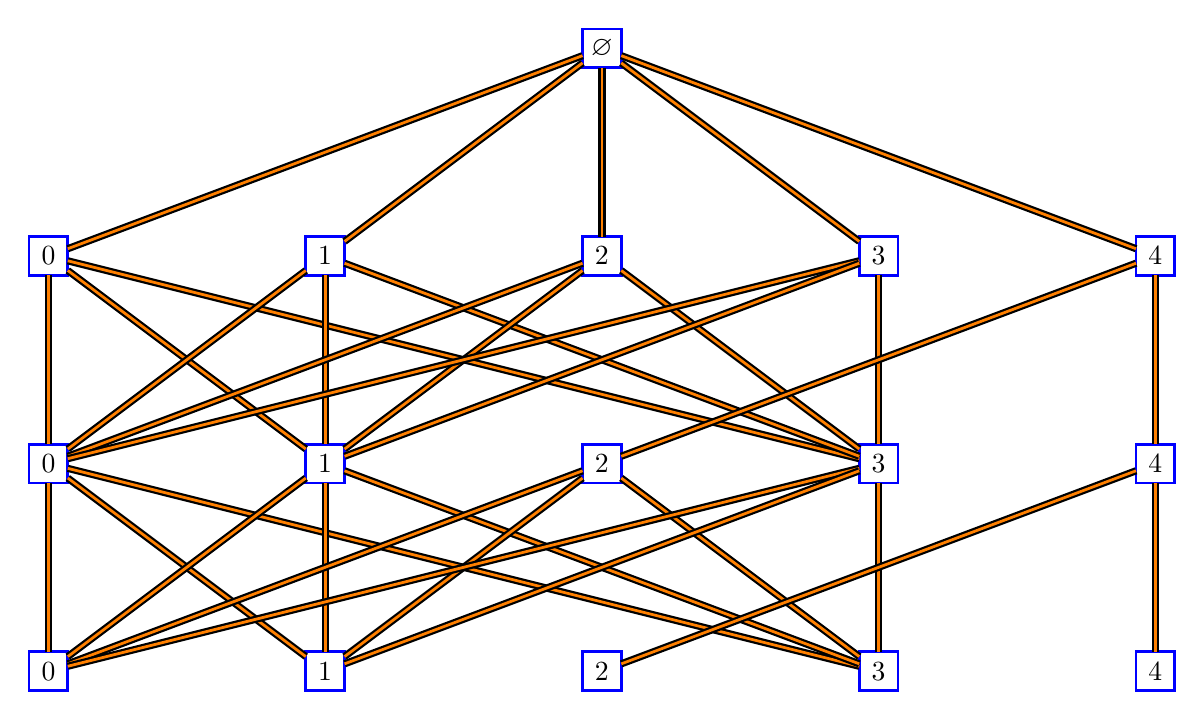
\begin{tikzpicture}[x=10pt,y=6pt]
  \centering
  \tikzset{VertexStyle/.style = {
    shape         = rectangle,
    draw          = blue, 
    fill          = white, 
  	line width    = 1pt, 
    text          = black,
    inner sep     = 1pt,
    outer sep     = 0pt,
    minimum size  = 14 pt,
    scale         = 1
    }
  }
  \tikzset{EdgeStyle/.style = {
    draw            = black, 
    thick,
    double          = orange,
    double distance = 1pt
    }
  }
  \tikzset{EdgeLabelStyle/.style = {
    draw          = black,
  	shape         = circle, 
  	line width    = 1pt, 
  	minimum size  = 10pt, 
    inner sep     = 1pt,
    outer sep     = 0pt,
    fill          = yellow,
    text          = black,
    scale         = 1
    }
  }

	\node[VertexStyle](A1) at (25, 43.75) {$\varnothing$};
	\node[VertexStyle](B1) at (5, 31.25) {$0$};
	\node[VertexStyle](B2) at (15, 31.25) {$1$};
	\node[VertexStyle](B3) at (25, 31.25) {$2$};
	\node[VertexStyle](B4) at (35, 31.25) {$3$};
	\node[VertexStyle](B5) at (45, 31.25) {$4$};
	\node[VertexStyle](C1) at (5, 18.75) {$0$};
	\node[VertexStyle](C2) at (15, 18.75) {$1$};
	\node[VertexStyle](C3) at (25, 18.75) {$2$};
	\node[VertexStyle](C4) at (35, 18.75) {$3$};
	\node[VertexStyle](C5) at (45, 18.75) {$4$};
	\node[VertexStyle](D1) at (5, 6.25) {$0$};
	\node[VertexStyle](D2) at (15, 6.25) {$1$};
	\node[VertexStyle](D3) at (25, 6.25) {$2$};
	\node[VertexStyle](D4) at (35, 6.25) {$3$};
	\node[VertexStyle](D5) at (45, 6.25) {$4$};
	\draw[EdgeStyle](A1) to (B1);
	\draw[EdgeStyle](A1) to (B2);
	\draw[EdgeStyle](A1) to (B3);
	\draw[EdgeStyle](A1) to (B4);
	\draw[EdgeStyle](A1) to (B5);
	\draw[EdgeStyle](B1) to (C1);
	\draw[EdgeStyle](B1) to (C2);
	\draw[EdgeStyle](B1) to (C4);
	\draw[EdgeStyle](B2) to (C1);
	\draw[EdgeStyle](B2) to (C2);
	\draw[EdgeStyle](B2) to (C4);
	\draw[EdgeStyle](B3) to (C1);
	\draw[EdgeStyle](B3) to (C2);
	\draw[EdgeStyle](B3) to (C4);
	\draw[EdgeStyle](B4) to (C1);
	\draw[EdgeStyle](B4) to (C2);
	\draw[EdgeStyle](B4) to (C4);
	\draw[EdgeStyle](B5) to (C3);
	\draw[EdgeStyle](B5) to (C5);
	\draw[EdgeStyle](C1) to (D1);
	\draw[EdgeStyle](C1) to (D2);
	\draw[EdgeStyle](C1) to (D4);
	\draw[EdgeStyle](C2) to (D1);
	\draw[EdgeStyle](C2) to (D2);
	\draw[EdgeStyle](C2) to (D4);
	\draw[EdgeStyle](C3) to (D1);
	\draw[EdgeStyle](C3) to (D2);
	\draw[EdgeStyle](C3) to (D4);
	\draw[EdgeStyle](C4) to (D1);
	\draw[EdgeStyle](C4) to (D2);
	\draw[EdgeStyle](C4) to (D4);
	\draw[EdgeStyle](C5) to (D3);
	\draw[EdgeStyle](C5) to (D5);

  \end{tikzpicture}

\end{document}
